\documentclass[11pt,a4paper]{report}

\usepackage[margin=2.2cm]{geometry}
\usepackage{titlesec}
\usepackage{enumitem}
\usepackage{longtable}
\usepackage{array}
\usepackage{booktabs}
\usepackage{xcolor}
\usepackage{listings}
\usepackage{hyperref}
\usepackage{tikz}
\usepackage{tcolorbox}
\usepackage{fancyhdr}
\usepackage{parskip}
\usetikzlibrary{positioning,arrows.meta,shapes.geometric,fit,backgrounds}

\definecolor{codebg}{RGB}{245,245,245}
\definecolor{hpegreen}{RGB}{1,169,130}
\definecolor{darknavy}{RGB}{30,40,60}

\lstset{
  backgroundcolor=\color{codebg},
  basicstyle=\ttfamily\small,
  breaklines=true,
  frame=single,
  numbers=left,
  numberstyle=\tiny,
  columns=fullflexible,
  showstringspaces=false
}

\hypersetup{
  colorlinks=true,
  linkcolor=darknavy,
  urlcolor=hpegreen,
  citecolor=hpegreen
}

\pagestyle{fancy}
\fancyhf{}
\fancyhead[L]{ArchGuide Interview Preparation - Volume 1}
\fancyhead[R]{\thepage}
\renewcommand{\headrulewidth}{0.4pt}

\titleformat{\chapter}[display]
  {\normalfont\huge\bfseries\color{darknavy}}
  {\chaptertitlename\ \thechapter}{20pt}{\Huge}

\newtcolorbox{notebox}[1][]{colback=hpegreen!8,colframe=hpegreen!60!black,fonttitle=\bfseries,title={#1}}
\newtcolorbox{qabox}[1][]{colback=darknavy!5,colframe=darknavy!70,fonttitle=\bfseries,title={#1}}

\title{\Huge \textbf{ArchGuide Project} \\[0.4cm] \Large Complete Reverse-Engineering and Interview Preparation Guide \\[0.6cm] \large Volume 1 of 3: Architecture, Tech Stack, Folder Structure, Codebase, Frontend, Backend and Database Deep Dive}
\author{Prepared for Full-Time Offer Technical Interview Preparation \\ Hewlett Packard Enterprise (HPE)}
\date{\today}

\begin{document}

\maketitle

\tableofcontents

\chapter{Executive Summary}

\section{What Problem This Project Solves}

Organizations that want to build AI powered applications on top of their own data face a recurring and expensive decision early in the design process: which architectural pattern should be used to connect a Large Language Model (LLM) to proprietary information. The four common patterns are:

\begin{itemize}[leftmargin=*]
  \item \textbf{Retrieval Augmented Generation (RAG)}: store documents as vector embeddings, retrieve the most relevant chunks at query time, and feed them to the LLM as context.
  \item \textbf{Fine-Tuning}: retrain or adapt the weights of a base model on a domain specific dataset so that the model internalizes the knowledge.
  \item \textbf{Context Augmented Generation (CAG)}: load an entire (typically small and static) knowledge base directly into the model context window for every query, avoiding a retrieval step altogether.
  \item \textbf{Hybrid}: combine two or more of the above, for example fine-tuning a model for domain vocabulary while also using retrieval for up to date facts.
  \end{itemize}

Choosing incorrectly is costly: RAG pipelines built for static, small, highly specialized data may be more complex and expensive than necessary; fine-tuning a model for fast changing data leads to constant retraining costs and stale knowledge; CAG used on a huge or rapidly changing corpus blows the context window and the budget. Most teams make this decision informally, based on whichever pattern is currently fashionable, rather than on a rigorous evaluation of their actual requirements (data size, change frequency, latency needs, accuracy requirements, domain specificity, security constraints, cost sensitivity, deployment environment, and expected user scale).

ArchGuide solves this problem by turning the architecture selection decision into a structured, evidence based, repeatable process. A user either uploads a requirements document (a project brief, a system design document, an RFP, a product specification) or answers a short guided questionnaire. The system extracts ten well defined "signals" from that input, scores all four architecture patterns against those signals using a transparent and deterministic rule engine, and returns a ranked recommendation complete with a confidence score, a sensitivity analysis (how fragile the recommendation is to changes in any one signal), a cost estimate in Indian Rupees for each architecture, and a downloadable PDF report suitable for sharing with stakeholders.

\section{Why the Project Exists}

The project exists to remove guesswork from a high stakes engineering decision and to make that decision auditable. Instead of an architect saying "I think we should use RAG because that is what everyone uses," ArchGuide produces a defensible, signal by signal breakdown: "Your dataset is very large (signal: dataset\_size = very\_large, confidence 0.82, extracted from page 3), your data changes daily (signal: data\_volatility = high, confidence 0.91), and your accuracy requirement is very high (confidence 0.77). Based on these signals, RAG scores 78/100, Fine-Tuning scores 41/100, and the recommended architecture is RAG because it can incorporate new information without retraining and grounds answers in source documents, which directly addresses your stated accuracy requirement." This is the kind of reasoning a senior architect would produce manually after hours of analysis; ArchGuide produces it in minutes and makes the reasoning chain fully traceable back to the source text.

\section{Who the Target Users Are}

\begin{itemize}[leftmargin=*]
  \item \textbf{Solutions architects and technical leads} who need to justify an architecture choice to stakeholders or in a design review.
  \item \textbf{Engineering managers and product managers} who are not deeply technical but need to understand the tradeoffs between approaches before committing budget.
  \item \textbf{Students and early career engineers} who want to learn, in a guided and example driven way, how the four architecture patterns differ and which signals drive the choice between them.
  \item \textbf{Consulting teams} that repeatedly need to produce architecture recommendation reports for different clients and want a consistent, explainable methodology plus a polished exportable artifact (the PDF report).
\end{itemize}

\section{What Business Value It Creates}

\begin{itemize}[leftmargin=*]
  \item \textbf{Reduces decision risk}: a wrong architecture choice discovered after months of implementation is extremely expensive to reverse; ArchGuide front loads the analysis.
  \item \textbf{Saves senior engineering time}: the manual version of this analysis (reading a requirements document, mapping it to architecture tradeoffs, writing a recommendation memo) can take a senior engineer half a day; ArchGuide compresses this into minutes while remaining transparent about its reasoning.
  \item \textbf{Produces shareable artifacts}: the PDF export (analysis report and cost report) can be attached directly to a design document or sent to a client, with all numbers traceable to extracted evidence.
  \item \textbf{Provides cost transparency early}: the cost analysis (in INR, broken down by compute, storage, inference, networking, security and maintenance) lets a team budget before committing to an approach.
  \item \textbf{Creates a feedback loop}: the follow up questionnaire lets a user correct or supplement low confidence signals, and the system re-scores instantly, turning architecture selection into an interactive conversation rather than a one shot guess.
\end{itemize}

\section{What Makes the Solution Unique}

\begin{enumerate}[leftmargin=*]
  \item \textbf{Determinism and explainability over black box machine learning}: the scoring engine is a hand authored rule matrix (signal value to architecture score deltas), not a trained classifier. Every number in the final recommendation can be traced to a specific rule and a specific extracted signal. This is a deliberate engineering tradeoff favoring auditability over the theoretical accuracy gains of a learned model, and it is one of the most defensible design decisions in the project (see Chapter on Engineering Tradeoffs in Volume 2).
  \item \textbf{Hybrid extraction pipeline}: signals are extracted using both an LLM (for nuanced natural language understanding) and a deterministic keyword and regex heuristic engine (for resilience when the LLM is unavailable, slow, or returns malformed output). This dual path design means the system degrades gracefully instead of failing outright.
  \item \textbf{Source verification and anti-hallucination guards}: every signal extracted by the LLM is checked against the original document text (with fuzzy matching for paraphrased quotes), and any signal whose value does not match a known scoring rule key is nulled out rather than silently accepted. This directly defends against LLM hallucination, a major real world concern in production LLM systems.
  \item \textbf{Sensitivity analysis}: the system does not just say "RAG is the answer"; it tells the user how stable that answer is, for example "if your data volatility were actually low instead of high, the recommendation would flip to CAG." This is unusual in consumer facing AI tools and demonstrates a first principles understanding of decision robustness.
  \item \textbf{Dual entry workflows}: a user can either upload an unstructured document (harder, requires parsing, relevance gating, and extraction) or fill out a structured questionnaire (easier, more reliable, but requires the user to already know the answers). Both paths converge on the same scoring engine.
  \item \textbf{Production hardening}: the codebase contains an unusually large number of explicitly tagged security and performance fixes (prefixed SEC, B, AI, P7, AUTH, FE in code comments), indicating that this was iterated on with attention to real world failure modes such as cache poisoning across users, path traversal in file uploads, JWT impersonation, rate limiting, orphaned session recovery after crashes, and event loop starvation from slow external calls.
\end{enumerate}

\chapter{Project Overview}

\section{Project Goal}

To build an end to end web application that takes either an unstructured requirements document or a structured questionnaire as input, and outputs a ranked, explainable, cost aware recommendation for which AI system architecture (RAG, Fine-Tuning, CAG, or Hybrid) best fits the stated requirements, while allowing the user to interactively refine the recommendation and export it as a professional PDF report.

\section{Main Features}

\begin{enumerate}[leftmargin=*]
  \item \textbf{User authentication} via Firebase (Google sign in), with a guest mode that allows full use of the product without an account (using a locally generated guest identifier).
  \item \textbf{Project management}: users can create, rename, duplicate, and delete named "projects," each of which can contain one or more analysis runs, with full history tracking.
  \item \textbf{Document upload analysis}: upload a PDF, DOCX, or TXT file; the system parses it, validates that it is actually an architecture relevant document (rejecting things like invoices or screenshots), extracts ten signals using an LLM plus heuristic fallback, indexes the document into a vector database for retrieval augmented extraction, and produces a full recommendation.
  \item \textbf{Guided questionnaire analysis}: answer up to ten multiple choice questions about the project's requirements; the system converts the answers directly into signals (bypassing document parsing) and produces a recommendation.
  \item \textbf{Architecture recommendation}: a ranked list of all four architectures with numeric scores (0 to 100), an overall confidence score, a natural language explanation of why the top choice was selected and why the others were not, and a "suitability" classification (Highly Suitable, Suitable, Moderately Suitable, Not Recommended) for each.
  \item \textbf{Sensitivity analysis}: identifies which extracted signals are "fragile," meaning that a small change in their value would change the final recommendation, and reports a numeric stability score.
  \item \textbf{Cost analysis}: an India specific (INR) cost projection for each architecture, broken down by compute, storage, API and inference, networking, security premium, and maintenance multiplier, with monthly, annual, and per query estimates, plus an efficiency ranking that divides suitability by cost.
  \item \textbf{Follow up questionnaire}: for any signal that was extracted with low confidence or not extracted at all, the system generates a targeted multiple choice question; answering it triggers an instant re-score without reprocessing the original document.
  \item \textbf{PDF export}: two distinct downloadable PDF reports (a full analysis report and a dedicated cost report), generated server side with custom layout code (not a generic template engine), suitable for sharing with non-technical stakeholders.
  \item \textbf{AI chat assistant}: a floating chat widget, scoped to the specific analysis result, that can answer follow up questions about the recommendation using a streaming LLM response, with a hardcoded safety filter that refuses to reveal system internals, API keys, or prompts (a defense against prompt injection and information disclosure).
  \item \textbf{Decision trace and pipeline visualization}: a step by step, timestamped log of every stage the analysis pipeline went through (parsing, relevance check, vector indexing, signal extraction, scoring), shown to the user both during processing (as a live progress indicator) and after completion (as an audit trail).
  \item \textbf{Analysis history}: each project keeps a local record of its past analysis runs, letting a user compare how the recommendation changed as they refined their inputs.
\end{enumerate}

\section{User Journey (End to End Workflow)}

\begin{enumerate}[leftmargin=*]
  \item The user lands on the marketing home page, which explains the four architecture patterns and the value proposition, and clicks through to the projects dashboard.
  \item The user is optionally prompted to sign in with Google (Firebase Authentication); they may also skip and continue as a guest, in which case a random guest identifier is generated and stored in the browser's local storage.
  \item The user creates a new project (giving it a name and description) or opens an existing one.
  \item Inside a project, the user chooses between two analysis modes: "Upload a document" or "Answer a guided questionnaire," and optionally selects an LLM provider (OpenAI or Groq).
  \item \textbf{Document path}: the user drags and drops or selects a file (PDF, DOCX, or TXT, up to 50 MB). The frontend uploads it with a bearer token (if signed in) to the backend, which creates a database session row, parses the document, validates relevance, indexes it into the Qdrant vector store, extracts signals (LLM plus heuristic fallback, with confidence gating and concentration warnings), scores the four architectures, computes sensitivity and cost analyses, generates follow up questions for weak signals, and persists the final result.
  \item \textbf{Questionnaire path}: the user answers up to ten multiple choice questions; the frontend submits the answers directly; the backend converts them straight into signals (skipping parsing and extraction entirely) and runs the same scoring, sensitivity, cost, and follow up generation steps.
  \item While processing, the results page shows a staged progress indicator (Parsing, Extracting Signals, Scoring, Validating for documents; a shorter synchronous flow for questionnaires) with elapsed time and a live activity log driven by the backend's decision trace, polling the backend with an exponentially increasing interval to avoid hammering the server.
  \item Once complete, the results page renders: the recommended architecture with its description and confidence; a bar chart of all four architecture scores; a radar chart of factor level scores; the extracted signals with their confidence, source quotes, and page numbers; a sensitivity analysis panel; a cost analysis panel with charts and INR figures; any follow up questions (which the user can answer to refine the result, triggering an immediate re-score); a sidebar showing the decision pipeline ranking and the full decision trace; and a floating chat assistant scoped to this analysis.
  \item The user can download either a full analysis PDF or a cost analysis PDF, both generated on the backend and streamed to the browser.
  \item The user can return to the project dashboard, see a history of past analyses for that project, edit the project, duplicate it, or delete it (with an undo window).
  \item If the user was browsing as a guest and later signs in, the application offers to transfer their guest projects to their authenticated account, with collision detection on project names.
\end{enumerate}

\section{Real World Use Cases}

\begin{itemize}[leftmargin=*]
  \item A solutions architecture team at an enterprise receives a new client's requirements document and needs an initial, defensible recommendation before the kickoff meeting.
  \item A startup's technical co-founder is choosing between building a RAG based support bot or fine-tuning a model on historical support tickets, and wants a structured comparison with cost estimates before pitching to investors.
  \item A graduate student studying applied machine learning systems wants to understand, through guided examples, how dataset size, volatility, and accuracy requirements interact to favor one architecture pattern over another.
  \item A consulting firm needs to produce consistent, professional looking architecture recommendation reports for multiple clients without re-deriving the analysis methodology each time.
\end{itemize}

\section{High Level Workflow Diagram}

\begin{center}
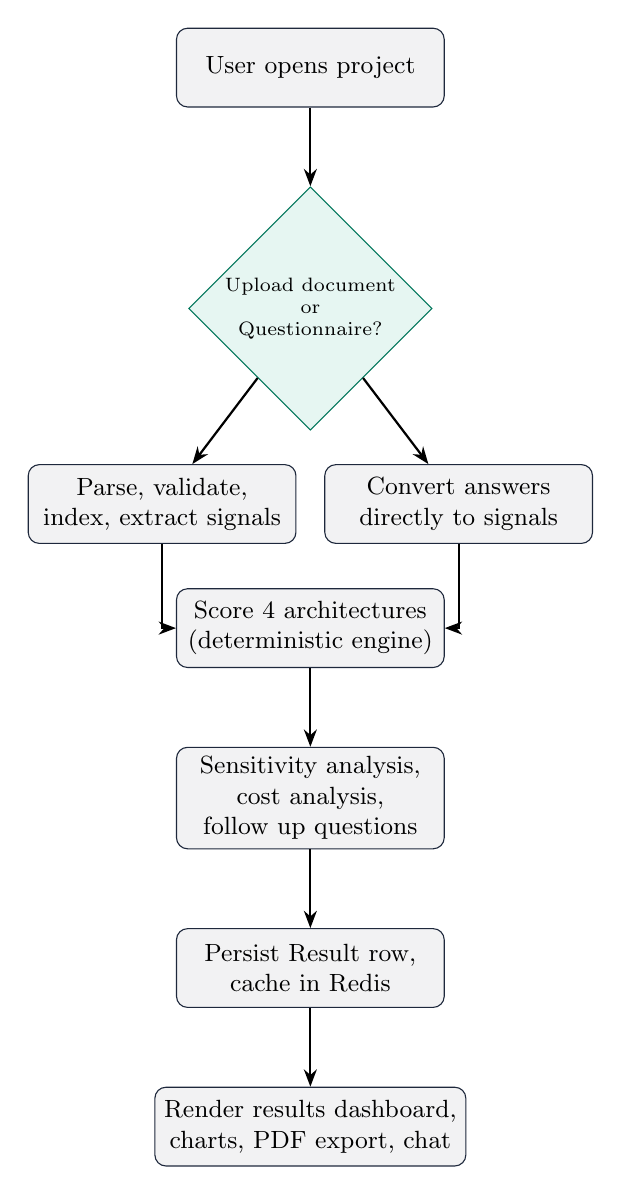
\begin{tikzpicture}[
  node distance=10mm and 14mm,
  box/.style={rectangle, rounded corners, draw=darknavy, fill=darknavy!6, align=center, minimum width=34mm, minimum height=10mm, font=\small},
  decision/.style={diamond, draw=hpegreen!70!black, fill=hpegreen!10, align=center, font=\scriptsize, inner sep=1pt, minimum width=26mm},
  arrow/.style={-{Stealth[length=2.2mm]}, thick}
]
\node[box] (start) {User opens project};
\node[decision, below=of start] (mode) {Upload document\\or\\Questionnaire?};
\node[box, below left=12mm and -6mm of mode] (upload) {Parse, validate,\\index, extract signals};
\node[box, below right=12mm and -6mm of mode] (quest) {Convert answers\\directly to signals};
\node[box, below=20mm of mode] (score) {Score 4 architectures\\(deterministic engine)};
\node[box, below=of score] (extra) {Sensitivity analysis,\\cost analysis,\\follow up questions};
\node[box, below=of extra] (persist) {Persist Result row,\\cache in Redis};
\node[box, below=of persist] (display) {Render results dashboard,\\charts, PDF export, chat};

\draw[arrow] (start) -- (mode);
\draw[arrow] (mode) -- (upload);
\draw[arrow] (mode) -- (quest);
\draw[arrow] (upload) |- (score);
\draw[arrow] (quest) |- (score);
\draw[arrow] (score) -- (extra);
\draw[arrow] (extra) -- (persist);
\draw[arrow] (persist) -- (display);
\end{tikzpicture}
\end{center}

\chapter{System Architecture}

\section{Architecture Style}

ArchGuide follows a classic three tier web application architecture with an additional, clearly separated AI processing pipeline layer:

\begin{enumerate}[leftmargin=*]
  \item \textbf{Presentation tier}: a Next.js (App Router) single page application, server side rendered where helpful, client interactive where needed.
  \item \textbf{Application tier}: a FastAPI (Python, asynchronous) backend exposing a versioned REST API, containing routers, services, and a multi stage AI processing pipeline.
  \item \textbf{Data tier}: PostgreSQL (hosted on Supabase) for relational, durable data; Redis (hosted on Upstash) for ephemeral caching; Qdrant Cloud for vector embeddings used in retrieval augmented signal extraction.
\end{enumerate}

It is not a microservices architecture. It is a modular monolith: one deployable backend service containing clearly separated routers and services, communicating with several managed external systems (database, cache, vector store, authentication provider, LLM providers). This is an intentional and defensible choice for the project's current scale, discussed at length in the Engineering Tradeoffs chapter of Volume 2.

\section{Component Diagram}

\begin{center}
\begin{tikzpicture}[
  node distance=8mm and 10mm,
  comp/.style={rectangle, rounded corners, draw=darknavy, fill=white, align=center, minimum width=32mm, minimum height=11mm, font=\scriptsize, drop shadow},
  ext/.style={rectangle, rounded corners, draw=hpegreen!70!black, fill=hpegreen!8, align=center, minimum width=30mm, minimum height=11mm, font=\scriptsize},
  grp/.style={rectangle, rounded corners, draw=darknavy!40, dashed, inner sep=4mm},
  arrow/.style={-{Stealth[length=2mm]}, thick}
]

\node[comp] (browser) {Browser\\(Next.js client app)};
\node[comp, right=28mm of browser] (frontend) {Next.js Server\\(SSR + API routes)};
\node[comp, below=14mm of frontend] (backend) {FastAPI Backend\\(/api/v1, async)};

\node[ext, below left=16mm and -6mm of backend] (postgres) {PostgreSQL\\(Supabase)};
\node[ext, below=16mm of backend] (redis) {Redis\\(Upstash cache)};
\node[ext, below right=16mm and -6mm of backend] (qdrant) {Qdrant Cloud\\(vector store)};

\node[ext, above right=6mm and 18mm of backend] (llm) {LLM Providers\\(OpenAI / Groq / Ollama)};
\node[ext, above=14mm of browser] (firebase) {Firebase Auth\\(Google sign in)};

\draw[arrow] (browser) -- node[above,font=\tiny]{HTTPS} (frontend);
\draw[arrow] (frontend) -- node[right,font=\tiny]{REST / SSE} (backend);
\draw[arrow] (browser) -- node[left,font=\tiny]{ID token} (firebase);
\draw[arrow] (firebase) |- node[above,font=\tiny]{verify JWT} (backend);
\draw[arrow] (backend) -- node[left,font=\tiny]{SQL (psycopg2)} (postgres);
\draw[arrow] (backend) -- node[right,font=\tiny]{cache get/set} (redis);
\draw[arrow] (backend) -- node[right,font=\tiny]{embed / search} (qdrant);
\draw[arrow] (backend) -- node[above,font=\tiny]{generate / stream} (llm);
\end{tikzpicture}
\end{center}

\section{Component Responsibilities}

\subsection{Browser / Next.js Client Application}
\textbf{Why it exists:} provides the interactive user interface; renders charts, forms, progress indicators, and the chat widget; manages local state such as guest identifiers, project lists, and analysis history.
\textbf{Responsibility:} all user facing rendering and interaction; calling the backend REST API; managing the Firebase authentication SDK; client side routing between the landing page, project dashboard, analysis input page, and results page.
\textbf{Communication:} talks to the backend exclusively over HTTPS using `fetch`, including a streaming `EventSource`-style connection for the chat assistant; talks to Firebase directly for authentication.

\subsection{FastAPI Backend}
\textbf{Why it exists:} centralizes all business logic, the AI processing pipeline, data persistence, and security enforcement in one place that can be reasoned about, tested, and scaled independently of the frontend.
\textbf{Responsibility:} expose a versioned REST API (`/api/v1`); validate and authenticate every request; orchestrate the multi stage analysis pipeline (parse, validate, index, extract, score, persist); manage caching; generate PDF reports; stream chat responses; enforce rate limits and security headers; recover from crashes (orphaned session cleanup on startup).
\textbf{Communication:} synchronous SQL to PostgreSQL through SQLAlchemy and psycopg2; key-value operations to Redis; vector upsert and search calls to Qdrant Cloud; HTTP calls to LLM providers (OpenAI, Groq, or a local Ollama instance); JWT verification calls to the Firebase Admin SDK.

\subsection{PostgreSQL (Supabase)}
\textbf{Why it exists:} the system of record for all durable, relational data: users, projects, analysis sessions, extracted signals, and final results. A relational database was chosen because the data has clear relationships (a user has projects, a project has sessions, a session has signals and one result) and because transactional guarantees matter (an analysis result must be persisted atomically and consistently with its signals).
\textbf{Responsibility:} durable storage with foreign key integrity, cascading deletes, and indexing for fast lookups.
\textbf{Communication:} accessed only by the backend, never directly by the frontend, through a pooled, synchronous SQLAlchemy engine.

\subsection{Redis (Upstash)}
\textbf{Why it exists:} the AI pipeline (parsing, vector indexing, LLM calls, scoring) is the slowest and most expensive part of the system. Caching its outputs avoids redundant work when a user reloads a results page, when multiple backend workers handle requests for the same session, or when the same document is uploaded twice.
\textbf{Responsibility:} short lived caches for extracted signals (ten minute TTL), final results (fifteen minute TTL), and a separate two tier extraction cache keyed by document content hash (one hour TTL, with an in process LRU layer in front of Redis).
\textbf{Communication:} accessed only by the backend; the system is explicitly designed to degrade gracefully (return `None` and fall through to the database or to recomputation) if Redis is unreachable.

\subsection{Qdrant Cloud (Vector Store)}
\textbf{Why it exists:} to support retrieval augmented signal extraction, the system needs to find the most relevant passages of a (potentially very long) document for each of the ten signal categories, without sending the entire document to the LLM on every call. A vector database makes semantic similarity search over document chunks fast and persistent.
\textbf{Responsibility:} store chunk level embeddings tagged with a session identifier (for multi tenant isolation), and return the top matching chunks for a query embedding using cosine similarity.
\textbf{Communication:} accessed only by the backend's vector service; embeddings are generated by the embeddings utility (OpenAI or Ollama) before being upserted or searched.

\subsection{Firebase Authentication}
\textbf{Why it exists:} implementing a secure authentication system (password hashing, OAuth flows, session/token issuance, account recovery) from scratch is a large undertaking with significant security risk; Firebase Authentication is a managed, audited, industry standard service that handles this for free at the project's scale.
\textbf{Responsibility:} Google sign in flow on the client; issuing signed ID tokens (JWTs); the backend verifies these tokens using the Firebase Admin SDK to authenticate API requests.
\textbf{Communication:} the browser talks to Firebase directly for sign in; the backend talks to Google's public key infrastructure (through the Admin SDK) to verify token signatures, never to the user's credentials.

\subsection{LLM Providers (OpenAI, Groq, Ollama)}
\textbf{Why it exists:} the core "intelligence" of the product, natural language understanding of unstructured requirements documents and conversational chat, requires a large language model. Multiple providers are supported to balance cost (Groq's free tier and local Ollama), quality (OpenAI's GPT-4o-mini), and resilience (automatic fallback if a preferred provider's key is absent).
\textbf{Responsibility:} generate text completions, JSON structured extractions, and streaming chat tokens; generate embeddings for vector indexing.
\textbf{Communication:} the backend's `LLMClient` abstraction wraps provider specific HTTP APIs behind a single async interface, with token counting (tiktoken) to avoid exceeding context windows, connection pooling, and hard timeouts to prevent a slow provider from stalling the entire event loop.

\chapter{Complete Tech Stack Deep Dive}

For each technology this chapter explains what it is, why it was chosen here, the realistic alternatives, its pros and cons in this context, and a short set of interview question and answer pairs.

\section{Next.js (App Router) and React}
\textbf{What it is:} Next.js is a React based framework that adds file system routing, server side rendering, static generation, and build tooling on top of React, a component based JavaScript library for building user interfaces.
\textbf{Why chosen:} the project needs a fast, SEO friendly landing page (server rendering helps here) and a highly interactive dashboard and results experience (client rendering and rich state management help there). Next.js's App Router lets both coexist in one codebase, with file based routing matching the natural page hierarchy (`/projects`, `/projects/[projectId]/analyze`, `/results/[analysisId]`).
\textbf{Alternatives:} plain React with React Router and a separate static host; Vue with Nuxt; Angular; SvelteKit.
\textbf{Pros:} large ecosystem, file based routing reduces boilerplate, built in image and font optimization, incremental adoption of server and client components, strong TypeScript support.
\textbf{Cons:} steeper learning curve around server versus client component boundaries, framework version churn (the project uses a very recent Next.js 16 and React 19), potential for over fetching if server components are not used carefully.

\begin{qabox}[Sample Interview Q and A]
\textbf{Q: Why did you choose Next.js instead of plain React?} \\
A: Plain React requires assembling routing, SSR, and build tooling separately. Next.js's App Router gave file based routing that mirrors the page hierarchy directly (projects, analyze, results), server rendering for the marketing landing page where first paint speed matters, and a unified deployment story on Vercel. For a project of this size, the convenience and conventions outweighed the additional learning curve of the server and client component model.
\end{qabox}

\section{TypeScript}
\textbf{What it is:} a statically typed superset of JavaScript that compiles to plain JavaScript, adding compile time type checking.
\textbf{Why chosen:} the application has a non trivial API contract (analysis results, signals, cost breakdowns, sensitivity results) that is shared conceptually between frontend and backend; TypeScript interfaces (defined in `lib/api.ts`) make this contract explicit and catch mismatches at compile time rather than at runtime in production.
\textbf{Alternatives:} plain JavaScript with PropTypes or JSDoc type annotations; Flow.
\textbf{Pros:} catches a large class of bugs before runtime, improves editor autocomplete and refactoring safety, documents the shape of data implicitly through types.
\textbf{Cons:} added build step and learning curve, types can drift from the actual backend response shape if not kept in sync manually (there is no shared schema generation between FastAPI and the frontend in this project, which is a real weakness discussed in Chapter 24 of Volume 3).

\section{Tailwind CSS}
\textbf{What it is:} a utility first CSS framework that provides low level classes (for example `flex`, `px-4`, `text-lg`) that are composed directly in markup rather than writing separate CSS files.
\textbf{Why chosen:} enables rapid, consistent styling without context switching between files, and pairs naturally with component based frameworks like React.
\textbf{Alternatives:} traditional CSS or SCSS modules, CSS-in-JS libraries (styled-components, Emotion), component libraries with their own styling systems (Material UI, Chakra UI).
\textbf{Pros:} fast iteration, small final CSS bundle through purging unused classes, consistent design tokens (spacing, color) across the app.
\textbf{Cons:} verbose markup ("class name soup"), requires discipline to avoid duplicated utility chains, less natural for highly themeable design systems compared to CSS variables with component libraries (mitigated here by `cn()` helper merging `clsx` and `tailwind-merge`).

\section{Framer Motion}
\textbf{What it is:} a production ready animation library for React that provides declarative animation primitives (`motion.div`, `useScroll`, `useTransform`).
\textbf{Why chosen:} the marketing landing page and several components rely on scroll driven and entrance animations (fade, scale, slide) to create a polished, modern feel; Framer Motion makes these declarative and performant (using the browser's animation APIs under the hood).
\textbf{Alternatives:} CSS animations and transitions directly, GSAP, react-spring.
\textbf{Pros:} declarative API that fits React's mental model, good performance, rich gesture and scroll integration.
\textbf{Cons:} adds bundle size, can be overused to the detriment of performance on lower end devices (the project mitigates this by skipping scroll animations on mobile).

\section{Recharts}
\textbf{What it is:} a charting library built on React and D3 that renders charts as SVG React components.
\textbf{Why chosen:} the results dashboard and cost analysis panels need bar charts (architecture score comparison, cost comparison) and a radar chart (factor level score breakdown); Recharts provides these as composable React components that integrate naturally with the app's data flow and theming.
\textbf{Alternatives:} Chart.js, D3.js directly, Victory, Nivo.
\textbf{Pros:} React native API, responsive containers, reasonable customization without raw D3 complexity.
\textbf{Cons:} can re-render expensively on frequent data updates (the project explicitly memoizes chart components to avoid excessive re-renders during result polling), less flexible than raw D3 for highly bespoke visualizations.

\section{Firebase Authentication}
\textbf{What it is:} a managed authentication service from Google that handles identity provider integration (in this project, Google sign in), issues signed JSON Web Tokens (JWTs) as ID tokens, and exposes a client SDK plus an Admin SDK for server side verification.
\textbf{Why chosen:} building a secure authentication system from scratch (password hashing, OAuth redirect handling, token issuance and rotation, account recovery flows) is both time consuming and a major source of security vulnerabilities if done incorrectly. Firebase provides a free, audited, industry standard solution, and its client SDK integrates cleanly with a React frontend while its Admin SDK integrates cleanly with a Python backend.
\textbf{Alternatives:} Auth0, Clerk, AWS Cognito, a custom JWT based system with a library such as `passlib` and `python-jose`.
\textbf{Pros:} no password storage liability for the application, free tier sufficient for the project's scale, mature client and server SDKs, built in protections against common authentication attacks.
\textbf{Cons:} vendor lock in (migrating away from Firebase later requires a user migration plan), less control over the exact authentication UX, the project must still implement its own authorization layer on top (Firebase only proves identity, not what a user is allowed to do).

\begin{qabox}[Sample Interview Q and A]
\textbf{Q: How does your backend trust a request as coming from an authenticated user?} \\
A: The frontend obtains a signed ID token (a JWT) from Firebase after the user signs in with Google, and sends it as a Bearer token in the Authorization header on every API request. The backend's `verify_firebase_token` dependency uses the Firebase Admin SDK to cryptographically verify the token's signature against Google's public keys and to check its expiry and audience claims, then extracts the user's UID from the verified claims. The backend never sees or stores the user's password; it only ever sees a short lived, signed, verifiable token. \\[4pt]
\textbf{Q: What happens if Firebase is down?} \\
A: New sign ins would fail, and any cached ID token would still work until its four minute client side cache expiry (and its underlying roughly one hour token expiry) elapsed; after that, authenticated requests would start failing verification. The application is explicitly designed so that guests can still use the full product without authentication, which limits the blast radius of a Firebase outage to authenticated only features such as project persistence tied to an account.
\end{qabox}

\section{FastAPI}
\textbf{What it is:} a modern, high performance Python web framework for building APIs, built on top of Starlette (ASGI) and Pydantic, with native support for asynchronous request handlers, automatic OpenAPI documentation, and dependency injection.
\textbf{Why chosen:} the backend needs to perform many I/O bound operations concurrently (calling LLM providers, querying the vector database, talking to Redis, serving multiple users), and Python's `async`/`await` model combined with FastAPI's native async support is a strong fit. FastAPI's Pydantic based request and response validation also gives the project automatic input validation and serialization with very little boilerplate.
\textbf{Alternatives:} Flask (synchronous by default, requires extensions for async and validation), Django REST Framework (heavier, more opinionated, less natively async), Node.js with Express or NestJS (different language ecosystem, would fragment the team's skill set if Python is preferred for the AI pipeline because of its library ecosystem).
\textbf{Pros:} excellent performance for I/O bound workloads, automatic request validation and response serialization through Pydantic, automatic interactive API documentation, first class async support, dependency injection that makes testing straightforward.
\textbf{Cons:} still a relatively young framework compared to Django or Flask (smaller, though rapidly growing, ecosystem of third party extensions), async code requires discipline (a single blocking call can stall the entire event loop, which the project explicitly guards against with `asyncio.wait_for` timeouts around LLM calls).

\section{SQLAlchemy and PostgreSQL (Supabase)}
\textbf{What they are:} SQLAlchemy is a Python SQL toolkit and Object Relational Mapper (ORM) that lets developers define database tables as Python classes and query them with Python expressions instead of raw SQL strings. PostgreSQL is a mature, open source relational database management system; Supabase is a managed hosting and tooling layer on top of PostgreSQL.
\textbf{Why chosen:} the application's data has clear relational structure (users own projects, projects contain sessions, sessions contain signals and produce one result) with foreign key relationships and the need for cascading deletes and transactional consistency; a relational database with an ORM is the natural fit. Supabase provides managed hosting, backups, and a generous free tier without the operational burden of running PostgreSQL directly.
\textbf{Alternatives:} a NoSQL document database such as MongoDB or Firestore (would require denormalizing relationships and handling consistency manually), a different managed Postgres provider (Neon, Railway, AWS RDS), a self hosted database.
\textbf{Pros:} strong consistency guarantees (ACID transactions), expressive query capability, mature tooling (Alembic for migrations), foreign key and cascade support enforced at the database level, JSONB columns available for semi structured data (used for the `Result` model's ranking, scores, and decision trace fields).
\textbf{Cons:} requires explicit schema migrations as the data model evolves (handled here with Alembic), vertical scaling limits compared to some NoSQL systems at extreme scale (not a concern at the project's current scale), synchronous driver (psycopg2) used here means database calls block the async event loop unless run in a thread pool, a real architectural tradeoff discussed further in Volume 2.

\begin{qabox}[Sample Interview Q and A]
\textbf{Q: Your backend is async (FastAPI) but your database driver (psycopg2) is synchronous. Is that a problem?} \\
A: It can be, because a blocking database call inside an async route handler will stall the entire event loop and prevent other requests from being served concurrently. FastAPI mitigates this by running synchronous dependency functions (such as the database session dependency) in a thread pool by default, so the event loop is not directly blocked, but this does add thread pool contention under high load. A fully async stack would use an async driver such as `asyncpg` with SQLAlchemy's async engine. This is a known tradeoff in the project: synchronous SQLAlchemy is simpler to write and debug, and at the project's current request volume the thread pool absorbs the blocking cost without issue, but it would be one of the first things to revisit when scaling toward tens of thousands of concurrent users.
\end{qabox}

\section{Alembic}
\textbf{What it is:} a database migration tool for SQLAlchemy that tracks incremental schema changes as versioned Python scripts.
\textbf{Why chosen:} as the data model evolved (for example, adding a `source_verified` column to the `Signal` table, or making datetime columns timezone aware), the project needed a reliable, repeatable, and reversible way to apply schema changes across environments (local development, testing, and production) without manual SQL.
\textbf{Alternatives:} hand written SQL migration scripts, Django's built in migration system (would require Django), no migrations at all (drop and recreate, which the project's `reset_db.py` script does for development convenience but which is unsafe for production).
\textbf{Pros:} versioned, auditable schema history; supports both upgrade and downgrade; integrates directly with SQLAlchemy models.
\textbf{Cons:} requires discipline to keep migration scripts and model definitions in sync; can be error prone with complex data migrations that mix schema changes and data transformations.

\section{Redis (Upstash) and the Caching Layer}
\textbf{What it is:} Redis is an in memory key value data store commonly used for caching, session storage, and pub/sub messaging. Upstash is a managed, serverless Redis hosting provider with a pay per request pricing model well suited to bursty workloads.
\textbf{Why chosen:} the AI pipeline's most expensive operations (document parsing, vector indexing, LLM based signal extraction, scoring) are deterministic for a given input, so their results can be safely cached and reused. Caching avoids redundant LLM API costs and dramatically speeds up repeated access to the same analysis (for example, when a user reloads the results page or when multiple backend worker processes serve requests for the same session).
\textbf{Alternatives:} Memcached (simpler, fewer data structures), an in process cache only (would not work across multiple worker processes or server restarts), no caching (would multiply LLM costs and latency).
\textbf{Pros:} very fast key value access, time to live (TTL) based expiry built in, shared across all backend worker processes (solving the multi worker cache consistency problem that a purely in process cache cannot solve), serverless pricing model fits a project without constant traffic.
\textbf{Cons:} adds an external dependency that can fail (mitigated here by graceful degradation: every cache lookup returns `None` on failure and the code falls through to recomputation or the database), cache invalidation is a classically hard problem (the project explicitly invalidates the signals cache when follow up answers change a session's signals, to avoid serving stale recommendations).

\section{Qdrant Cloud}
\textbf{What it is:} a managed vector database that stores high dimensional embedding vectors and supports fast approximate nearest neighbor search, typically using cosine similarity or other distance metrics.
\textbf{Why chosen:} to perform retrieval augmented signal extraction efficiently on long documents, the system needs to find which passages of a document are most relevant to each of the ten signal categories, without sending the entire document text to the LLM on every extraction call (which would be slow, expensive, and likely to exceed context window limits). A vector database makes this semantic search fast and persistent across requests and server restarts.
\textbf{Alternatives:} a local FAISS index (the project actually supports this as a fallback, see `faiss_store.py`, but FAISS indexes are not persisted across server restarts or shared across multiple worker processes by default), Pinecone, Weaviate, pgvector (a PostgreSQL extension that would keep everything in one database).
\textbf{Pros:} persistent storage that survives restarts, supports payload based filtering (used here to isolate each session's chunks from every other session's chunks, which is critical for multi tenant correctness and privacy), managed and scalable.
\textbf{Cons:} another external dependency and cost center, requires careful embedding dimension and distance metric configuration to match the embedding model in use, adds latency for the embed-then-search round trip.

\begin{qabox}[Sample Interview Q and A]
\textbf{Q: Why not just use pgvector and keep everything in PostgreSQL?} \\
A: That is a completely reasonable alternative and would reduce the number of external systems to manage. Qdrant was chosen here because it is purpose built for vector search, with optimizations (approximate nearest neighbor indexes, payload filtering, horizontal scaling) that a general purpose relational database extension does not match at larger scale. For this project's current document volume, pgvector would likely perform adequately and would be a legitimate simplification to consider; the choice of Qdrant reflects a decision to use a specialized tool for a specialized job and to keep that concern cleanly separated from the relational data model.
\end{qabox}

\section{LLM Providers: OpenAI, Groq, and Ollama}
\textbf{What they are:} OpenAI provides hosted large language models (the project uses `gpt-4o-mini`) through a paid API; Groq provides an extremely fast inference API for open models such as `llama-3.3-70b` with a usable free tier; Ollama is a tool for running open source language models locally on a developer's own machine (the project's default for local development, using small models such as `gemma3:1b`).
\textbf{Why chosen:} supporting multiple providers gives the project resilience (if one provider's API key is missing or the service is down, it falls back to another) and cost flexibility (Groq's free tier and local Ollama keep development and demo costs near zero, while OpenAI provides higher quality output for production use). The `provider` query parameter lets a user choose which to use per request.
\textbf{Alternatives:} committing to a single provider (simpler code, but a single point of failure and cost center), Anthropic's Claude API, open source self hosted inference servers such as vLLM or text-generation-inference.
\textbf{Pros:} resilience through provider diversity, cost control, ability to compare quality and latency across providers in the same product.
\textbf{Cons:} more code complexity (the `LLMClient` abstraction must normalize different APIs, error formats, and streaming protocols), inconsistent output quality and latency across providers can make user experience less predictable, prompt engineering must work reasonably well across multiple model families.

\begin{qabox}[Sample Interview Q and A]
\textbf{Q: What happens if the LLM call times out or returns garbage?} \\
A: Two layers of defense exist. First, every LLM call is wrapped in `asyncio.wait_for` with a ninety second timeout, so a stalled provider cannot block the event loop indefinitely; if it times out, the code treats it as a failure and falls through. Second, if the LLM based signal extraction returns zero usable signals (whether from a timeout, a malformed JSON response, or simply a model that could not find any signals), a completely independent heuristic extraction engine runs over the document text using more than ninety hand written regular expression rules with negation detection. This means the user always gets a result, just potentially with lower confidence scores, rather than a hard failure. \\[4pt]
\textbf{Q: How do you stop the LLM from echoing back something dangerous, like an API key or a system prompt, in the chat assistant?} \\
A: The chat router applies a hardcoded safety gate, `_is_unsafe()`, which uses regular expressions to detect requests that ask for API keys, system prompts, or backend implementation details, and returns a fixed refusal message before the request ever reaches the model. This is a defense in depth measure: even if the model itself would refuse such a request, the application does not rely on the model's own judgment for this class of information disclosure risk.
\end{qabox}

\section{tiktoken}
\textbf{What it is:} a fast, byte pair encoding based tokenizer library originally built for OpenAI's models, used to count how many tokens a piece of text will consume.
\textbf{Why chosen:} large language models have fixed context window sizes measured in tokens, not characters; sending a prompt that exceeds this limit causes an error or silent truncation by the provider. The project uses `tiktoken` to count tokens before sending a prompt, and truncates deterministically on the application side (preserving the most important parts of the prompt) rather than letting the provider truncate unpredictably, which would harm reproducibility.
\textbf{Alternatives:} estimating token counts from character counts (a rough approximation, error prone for non English text or code), provider specific tokenizer libraries.
\textbf{Pros:} accurate token counting that matches how the model will actually see the text, enables deterministic and controlled truncation.
\textbf{Cons:} `tiktoken`'s encodings are calibrated for OpenAI's models and are an approximation when used with other providers such as Groq or Ollama that may use different tokenizers internally.

\section{PyMuPDF (fitz) and python-docx}
\textbf{What they are:} PyMuPDF (imported as `fitz`) is a Python library for reading and manipulating PDF documents, including page level text extraction; `python-docx` is a library for reading and writing Microsoft Word `.docx` files.
\textbf{Why chosen:} the document upload feature must support the most common requirements document formats (PDF, DOCX, plain text); these libraries are the de facto standard, well maintained choices for parsing each format in Python, and PyMuPDF in particular provides reliable page level text extraction, which the project needs to report which page a signal's evidence came from.
\textbf{Alternatives:} `pdfplumber` or `PyPDF2` for PDFs (less robust text extraction in some cases), Apache Tika (a heavier, JVM based universal document parser), cloud document AI services (added cost and external dependency).
\textbf{Pros:} fast, accurate text extraction, page level granularity, broad format support within their respective domains.
\textbf{Cons:} text extraction quality from PDFs can vary significantly depending on how the PDF was generated (scanned image based PDFs without OCR will yield no extractable text, a known limitation), DOCX parsing in this project treats the entire document as a single page, which loses page level attribution for that format.

\section{FPDF (PDF Generation)}
\textbf{What it is:} a lightweight, pure Python library for generating PDF documents programmatically, by issuing drawing and layout commands (text, lines, rectangles, images) rather than rendering from HTML or a template engine.
\textbf{Why chosen:} the project needed full control over the visual layout of two distinct, polished, multi section PDF reports (the analysis report and the cost report), including custom color coded tables, progress bars, badges, and multi page flowing content. A low level drawing library gives precise control that a generic HTML to PDF converter would make harder to achieve consistently.
\textbf{Alternatives:} rendering HTML/CSS to PDF with a tool such as WeasyPrint or Puppeteer (easier to style with familiar web technologies, but heavier dependencies and less precise pagination control), a reporting framework such as ReportLab (more powerful but with a steeper learning curve), generating reports client side with a browser print dialog (less consistent across browsers and devices).
\textbf{Pros:} fine grained layout control, no headless browser dependency, predictable and consistent output, lightweight.
\textbf{Cons:} verbose code (every visual element is drawn with explicit coordinates and dimensions), harder to maintain and restyle than a templated approach, no automatic responsive layout (the project's `pdf_report.py` and `cost_report_pdf.py` contain large amounts of manual layout arithmetic).

\section{SlowAPI (Rate Limiting)}
\textbf{What it is:} a rate limiting library for Starlette and FastAPI, inspired by Flask-Limiter, that enforces request rate limits per client (commonly identified by IP address) using configurable time windows.
\textbf{Why chosen:} the AI pipeline endpoints are expensive (they call paid or rate limited external LLM APIs); without rate limiting, a single user or a malicious actor could exhaust the application's LLM quota, run up costs, or degrade service for everyone else. The project applies different limits per endpoint (for example, four uploads per minute, ten questionnaire submissions per minute, thirty analysis polls per minute).
\textbf{Alternatives:} implementing rate limiting manually with Redis counters, an API gateway with built in rate limiting (Kong, AWS API Gateway), Cloudflare or another edge level rate limiter.
\textbf{Pros:} simple decorator based API that integrates directly into FastAPI route definitions, configurable per route limits, works with the existing middleware stack.
\textbf{Cons:} IP based identification can be inaccurate behind shared NATs or proxies (a known general limitation of IP based rate limiting, not specific to this library), in memory storage by default would not share state across multiple worker processes (a real consideration for horizontal scaling, discussed in the Scalability chapter of Volume 2).

\section{Pydantic}
\textbf{What it is:} a Python data validation and settings management library that uses Python type annotations to define data schemas, validate incoming data, and serialize outgoing data.
\textbf{Why chosen:} FastAPI is built around Pydantic for request body validation, response serialization, and application configuration (`config.py` uses Pydantic's `BaseSettings`); this gives the project automatic, declarative validation with clear error messages and eliminates large amounts of manual type checking code.
\textbf{Alternatives:} marshmallow, manual validation with `if` statements and `dict` access, dataclasses with custom validation.
\textbf{Pros:} declarative schema definition that doubles as documentation, automatic validation and clear error messages, seamless FastAPI integration, settings management with environment variable support.
\textbf{Cons:} adds a layer of abstraction that must be understood to debug validation errors effectively, schema changes require careful coordination with the frontend's separately maintained TypeScript types (no shared code generation between the two).

\section{Vanta.js and Lenis}
\textbf{What they are:} Vanta.js is a library for adding animated 3D backgrounds (such as a network of moving particles) to web pages using Three.js; Lenis is a smooth scrolling library that replaces the browser's native scroll behavior with an interpolated, easing based scroll experience.
\textbf{Why chosen:} purely for visual polish on the marketing landing page, to create a modern, premium feeling first impression that differentiates the product from a plain, utilitarian dashboard.
\textbf{Alternatives:} CSS based animated gradients or particle effects, no animated background at all, `react-tsparticles`.
\textbf{Pros:} visually striking, configurable, runs on the GPU through WebGL.
\textbf{Cons:} adds meaningful bundle size and runtime cost (mitigated here through lazy loading, so the effect never blocks the largest contentful paint), can hurt performance on low end devices or battery powered devices, purely cosmetic and unrelated to the product's core value, representing a calculated tradeoff of polish versus lean performance.

\section{uuid (Universally Unique Identifiers)}
\textbf{What it is:} a standard for generating identifiers that are unique across space and time without central coordination, typically 128 bit values usually represented as 36 character hexadecimal strings.
\textbf{Why chosen:} the project needs identifiers for projects, sessions, and guest users that are guaranteed not to collide, can be generated client side (for guest identifiers, before any server interaction occurs) or server side, and do not leak sequential information (unlike auto incrementing integer IDs, which can reveal how many records exist or enable enumeration attacks).
\textbf{Alternatives:} database auto incrementing integer primary keys (simpler but leak ordering and count information, and cannot be generated client side without a round trip), nanoid (shorter, URL friendly identifiers).
\textbf{Pros:} collision resistant without coordination, can be generated on the client for guest mode, do not reveal record counts or ordering.
\textbf{Cons:} longer than integer IDs (minor storage and index size overhead), not human friendly to read or communicate verbally.

\chapter{Folder Structure Analysis}

\section{Top Level Layout}

\begin{lstlisting}[language=, basicstyle=\ttfamily\footnotesize]
Updated-Codebase/
|-- backend/                 FastAPI application, AI pipeline, tests, migrations
|-- frontend/                Next.js application, components, lib, tests
|-- tests/docs/              Curated sample documents for pipeline verification
|-- vercel.json              Deployment configuration for the frontend on Vercel
|-- README.md                Project level documentation
\end{lstlisting}

\textbf{Why this split exists:} the backend and frontend are independently deployable services with different languages, dependency managers, and lifecycles (Python and pip for the backend; Node.js and npm for the frontend). Separating them at the repository root makes this independence explicit, allows each to have its own configuration, ignore rules, and CI pipeline, and mirrors how they would be deployed in practice (the backend on a Python friendly host such as Railway, the frontend on Vercel).

\section{Backend Folder Structure}

\begin{lstlisting}[language=, basicstyle=\ttfamily\footnotesize]
backend/
|-- app/
|   |-- main.py              FastAPI app factory, middleware, lifespan, routers
|   |-- core/security.py     Firebase JWT verification dependency
|   |-- limiter.py           Shared SlowAPI rate limiter instance
|   |-- db/
|   |   |-- models.py        SQLAlchemy ORM models (User, Project, Session, Signal, Result)
|   |   |-- session.py       Engine, session factory, get_db dependency
|   |   |-- base.py          Declarative base class
|   |-- routers/             One file per resource: upload, analysis, questionnaire,
|   |                        projects, users, chat
|   |-- schemas/             Pydantic request/response schemas (project.py, session.py)
|   |-- services/            Cross cutting application services: caching, vector search,
|   |                        cost analysis, PDF generation, recommendation orchestration
|   |-- utils/               Embeddings generation, FAISS local vector store fallback
|-- services/                Core AI pipeline services: document_parser, signal_extractor,
|                            scoring_engine, llm_client, followup_generator, extraction_cache
|-- alembic/                 Database migration scripts and configuration
|-- tests/                   pytest suite: api, integration, security
|-- config.py                Centralized Pydantic settings
|-- main.py                  Thin entry point that runs the app
|-- requirements.txt         Python dependency manifest
|-- Dockerfile               Container build definition
|-- railway.toml             Railway deployment configuration
|-- clear_db.py / reset_db.py / diagnose_pipeline.py / verify_scoring.py
                             Standalone operational and diagnostic scripts
\end{lstlisting}

\textbf{Why `app/services` and `services` both exist:} this is a notable structural quirk worth understanding and being able to explain honestly in an interview. The top level `backend/services/` directory contains the core, document agnostic AI pipeline logic (parsing, extraction, scoring, LLM client, follow up generation, caching of extraction results), while `backend/app/services/` contains services that are more tightly coupled to the FastAPI application's persistence and delivery concerns (Redis caching of API level results, vector indexing orchestration, cost analysis, PDF report generation, and the recommendation orchestration that ties the pipeline to the database). In effect, `backend/services` is closer to a "domain logic" layer and `backend/app/services` is closer to an "application layer," but the boundary is not perfectly clean (for example, `signal_service.py` lives under `app/services` yet orchestrates the domain level `SignalExtractor`). A candidate should be able to say plainly that this naming is a minor organizational inconsistency that arose from incremental development, and that a cleanup pass would consolidate these into a single, clearly named services layer with explicit sub-packages (for example `services/pipeline/` and `services/app/`).

\textbf{Why `routers` are split by resource:} each router file (`upload.py`, `analysis.py`, `questionnaire.py`, `projects.py`, `users.py`, `chat.py`) corresponds to one REST resource or workflow. This mirrors FastAPI's recommended structure (`APIRouter` per resource, included into the main app with a shared prefix), keeps each file focused and independently testable, and makes it easy to find the code responsible for any given endpoint by its URL path.

\textbf{Why `alembic/` exists separately:} database migrations are versioned, ordered scripts that must be run in sequence against a real database; keeping them in a dedicated directory with their own configuration (`alembic.ini`, `env.py`) is the standard Alembic convention and keeps migration concerns (which touch the database directly and can be destructive if mishandled) clearly separated from application code.

\section{Frontend Folder Structure}

\begin{lstlisting}[language=, basicstyle=\ttfamily\footnotesize]
frontend/
|-- src/
|   |-- app/                 Next.js App Router pages and layouts (file based routing)
|   |   |-- page.tsx                     Marketing landing page
|   |   |-- layout.tsx                   Root layout: providers, navbar, footer
|   |   |-- template.tsx                 Page transition wrapper
|   |   |-- error.tsx                    Global error boundary page
|   |   |-- projects/page.tsx            Project dashboard
|   |   |-- projects/[projectId]/analyze/page.tsx   Analysis input (upload or questionnaire)
|   |   |-- results/[analysisId]/page.tsx           Results and analysis dashboard
|   |-- components/          Reusable React components (one file per component)
|   |   |-- hooks/           Custom React hooks (use-debounced-dimensions)
|   |-- lib/                 Framework agnostic logic: API client, auth, storage, utilities
|   |-- types/               Ambient TypeScript type declarations (vanta.d.ts)
|-- tests/                   Vitest test suite: components and unit
|-- public/                  Static assets (SVG icons)
|-- next.config.ts           Next.js build and optimization configuration
|-- tsconfig.json            TypeScript compiler configuration
|-- package.json             Node dependency manifest and scripts
\end{lstlisting}

\textbf{Why `app/` mirrors the URL structure:} Next.js's App Router uses the file system as the routing table; a folder named `projects/[projectId]/analyze` containing a `page.tsx` automatically becomes the route `/projects/:projectId/analyze`. This eliminates a separate routing configuration file and keeps the relationship between URL and code immediately visible.

\textbf{Why `components/` is flat rather than deeply nested:} with around twenty five components, a flat directory remains easy to navigate with an editor's fuzzy file finder; deep nesting would add directory traversal overhead without a corresponding organizational benefit at this scale. A natural next step as the project grows would be to group components by feature area (for example `components/results/`, `components/projects/`, `components/chat/`).

\textbf{Why `lib/` is separate from `components/`:} `lib/` contains framework agnostic logic, API clients, authentication context, local storage backed stores, and pure utility functions, none of which render UI. Separating "what the app knows how to do" (`lib`) from "how the app looks and reacts" (`components`) is a common and effective separation of concerns that also makes the `lib` layer easier to unit test in isolation (as the `tests/unit/` directory demonstrates).

\section{Tests Sample Document Directory}

The `tests/docs/` directory contains a deliberately curated set of markdown documents representing canonical scenarios: a perfect candidate for each of the four architectures, ambiguous and minimal edge cases, and several documents that should be rejected (too short, wrong document type, an ArchGuide generated report fed back into itself, low signal density, and a large stress test document). \textbf{Why it exists:} automated and manual verification of the signal extraction and scoring pipeline requires known, ground truth inputs with expected outputs; this directory is effectively a hand authored regression test fixture set, referenced by `verify_scoring.py` and `diagnose_pipeline.py`.

\chapter{Codebase Deep Dive}

This chapter walks through the most important modules, classes, and functions in the system, explaining their purpose, inputs and outputs, internal logic, complexity, design patterns, and likely interview questions. Time and space complexity are expressed with respect to meaningful inputs: $n$ for document length in characters, $k$ for the number of signals (a constant, ten), and $u$ for the number of users or records where relevant.

\section{SignalExtractor (backend/services/signal\_extractor.py)}

\textbf{Purpose:} given the text of a document (or retrieved relevant chunks of it), produce a value and a confidence score for each of the ten predefined signal categories, with a source quote and page number for traceability.

\textbf{Inputs:} full document text, page level text segments, an optional set of vector retrieved context chunks, and an LLM client instance.

\textbf{Outputs:} a dictionary mapping each of the ten signal names to a structured value containing `value`, `confidence`, `source_text`, and `page_number`.

\textbf{Internal logic, step by step:}
\begin{enumerate}[leftmargin=*]
  \item \textbf{Cache check:} compute a fingerprint that combines a hash of the extraction prompt template with a hash of the document text; look this up in the extraction cache. If found, return immediately. This makes repeated extraction of the same document, or extraction after a prompt change, both correct and fast.
  \item \textbf{Page filtering:} score each page by counting how many signal related keywords it contains (using pre-compiled regular expressions, a deliberate optimization, see below) and select only the highest scoring pages to send to the LLM, reducing token usage and cost.
  \item \textbf{Chunking for long documents:} if the filtered text exceeds roughly eight thousand characters, split it into overlapping five thousand character chunks and process them concurrently, bounded by an `asyncio.Semaphore(5)` so that at most five LLM calls are in flight at once (preventing rate limit errors and memory blowups).
  \item \textbf{Winner takes all merge:} for each signal, keep the result with the highest confidence across all chunks, since a signal might appear, with different apparent confidence, in multiple chunks.
  \item \textbf{Heuristic fallback:} if the LLM extraction yields zero usable signals (for example, due to a timeout or malformed JSON), run a deterministic, regex based heuristic engine with more than ninety hand authored rules across all ten signal categories. This engine includes negation detection (recognizing phrases like "no real time requirement" so they are not misclassified as indicating high volatility).
  \item \textbf{Source verification:} for every signal that includes a source quote, check whether that quote actually appears in the original document text; if not found verbatim, attempt a fuzzy match requiring at least sixty percent word overlap, to tolerate minor paraphrasing by the LLM, and mark the signal as `source_verified` accordingly. Verification failure does not reduce the signal's confidence (a deliberate choice to avoid penalizing signals that are substantively correct but loosely quoted).
  \item \textbf{Merging keyword and LLM results:} keyword based heuristic findings are used to boost confidence in agreement cases, while the LLM's findings take priority for the actual value when both exist.
  \item \textbf{Anti hallucination null check:} any signal whose value does not appear as a valid key in the scoring engine's rule table is set to null, preventing a hallucinated value (for example, a nonsensical dataset size category) from silently propagating into the scoring stage.
\end{enumerate}

\textbf{Time complexity:} dominated by the number of LLM calls, which is bounded by $\lceil n / 5000 \rceil$ chunks, parallelized up to five at a time; keyword scanning is $O(n \cdot k)$ in the worst case but reduced to effectively $O(n)$ by pre-compiling each keyword's regular expression once rather than recompiling it for every scan (this was an explicitly tagged optimization, "B-08," in the codebase).

\textbf{Space complexity:} $O(n)$ for holding the document text and its chunks in memory, plus $O(k)$ for the extracted signal dictionary.

\textbf{Design patterns used:} Strategy pattern (the LLM based and heuristic based extraction strategies are interchangeable and one falls back to the other), Template Method-like staged pipeline (cache, filter, extract, verify, merge, sanitize as a fixed sequence of stages), Memoization (the cache check at the start).

\begin{qabox}[Likely Interview Questions]
\textbf{Q: Why do you run both an LLM based extractor and a regex based heuristic extractor?} \\
A: They have complementary failure modes. The LLM understands nuance and context (for example, recognizing that "we expect to onboard a few hundred users initially, scaling to tens of thousands within a year" implies a medium-to-large user scale signal) but can be slow, can return malformed output, can be unavailable if a provider has an outage or the API key is missing, and can occasionally hallucinate values. The regex heuristic engine is fast, free, always available, and fully deterministic, but cannot understand nuance beyond the patterns it was explicitly written to match. Running the LLM first and falling back to heuristics only when the LLM yields nothing gives the best of both: high quality results when possible, and a guaranteed, if less nuanced, result when not. \\[4pt]
\textbf{Q: How do you prevent the LLM from making up information that is not in the document?} \\
A: Three mechanisms layered together: source verification (checking that the quoted evidence text actually exists in the document, with fuzzy matching for paraphrasing), an anti hallucination null check (rejecting any extracted value that does not match a known, valid category in the scoring rule table), and the relevance gate that runs even earlier in the pipeline (rejecting documents that are not actually architecture related before any extraction is attempted at all).
\end{qabox}

\section{ScoringEngine (backend/services/scoring\_engine.py)}

\textbf{Purpose:} convert a dictionary of extracted signals into a numeric, ranked, explainable comparison of the four candidate architectures, plus a sensitivity analysis describing how stable that ranking is.

\textbf{Inputs:} a dictionary of signal name to `{value, confidence}`.

\textbf{Outputs:} `{recommended, ranking, scores, factor_breakdown, why_not, suitability}` from `score()`, and `{is_stable, stability_score, instabilities}` from `sensitivity_analysis()`.

\textbf{Core algorithm:}
\begin{enumerate}[leftmargin=*]
  \item For every signal whose confidence exceeds a small threshold (0.1), look up a pre-authored score delta (a number between 0.0 and 1.0) for each of the four architectures from a hand built `SCORING_RULES` table indexed by `[signal_name][signal_value][architecture]`.
  \item Multiply that delta by an "effective weight" equal to the signal's importance weight (a constant per signal, for example data volatility is weighted 1.3, cost sensitivity 0.8) times the signal's extraction confidence. This means a highly important signal extracted with low confidence contributes less than a moderately important signal extracted with high confidence, a deliberate and defensible design choice.
  \item Sum these weighted contributions across all active signals for each architecture, then normalize to a 0 to 100 scale by dividing by the total weight applied.
  \item Apply two synergy bonus rules that capture genuine cross architecture tension that a simple linear sum would miss: a "Hybrid synergy bonus" (added when there are simultaneously strong, distinct signals pulling toward both RAG and Fine-Tuning, capturing the idea that genuinely conflicting requirements are exactly when a hybrid approach makes sense) and a "CAG synergy bonus" (added when the dataset is small, static, and has low query volume, which is precisely CAG's sweet spot because a small, stable corpus fits entirely inside a model's context window).
  \item Compute an overall confidence score as a blend: seventy percent the average per-signal confidence, and thirty percent the "coverage" (the fraction of the ten possible signals that were actually extracted with meaningful confidence). This reflects the intuition that a recommendation based on nine well extracted signals should be trusted more than one based on three, even if those three were each extracted with high confidence.
\end{enumerate}

\textbf{Sensitivity analysis algorithm:} for each signal currently in use, hypothetically substitute every other possible value it could have taken, recompute the full score, and check whether the top recommended architecture would change. Signals whose hypothetical substitution changes the recommendation are reported as "instabilities," each with the original value, the perturbed value, the resulting recommendation change, and the score delta. An overall `stability_score` and boolean `is_stable` summarize this. To avoid recomputing the (relatively expensive) scoring function dozens of times per analysis, results are cached in an `OrderedDict` based least recently used (LRU) cache keyed by a hash of the signal dictionary, with a maximum size that triggers eviction of the oldest entry in O(1) time.

\textbf{Time complexity:} the base scoring pass is $O(k)$ since there are a constant ten signals and four architectures (effectively $O(1)$ in practical terms, but expressed as $O(k)$ for generality). The sensitivity analysis is $O(k \cdot v)$ where $v$ is the average number of alternative values per signal (typically three to five), each requiring a full $O(k)$ rescoring, so roughly $O(k^2 \cdot v)$ in the worst case, bounded by the LRU cache to avoid repeated work across requests.

\textbf{Space complexity:} $O(k)$ for the rule tables (constant size, since $k$ is fixed at ten signals and four architectures), plus $O(c)$ for the LRU sensitivity cache where $c$ is the configured maximum cache size (one thousand entries).

\textbf{Design patterns used:} Strategy-like rule table lookup (behavior is data driven rather than encoded in conditional branches, making it easy to tune scores without changing code), Memoization with bounded LRU eviction, pure function design (the scoring function has no side effects and is fully deterministic given its inputs, which is what makes both caching and sensitivity analysis correct and tractable).

\begin{qabox}[Likely Interview Questions]
\textbf{Q: Why is the scoring engine rule based instead of a trained machine learning model?} \\
A: Explainability and auditability. Every single point in a final score can be traced back to a specific signal, its extracted value, its confidence, and a specific, hand authored rule. This is essential for a tool whose entire purpose is to help a human justify an architecture decision to other humans; "the model said so" is not an acceptable answer in a design review, but "your data changes daily, which scores 0.85 toward RAG because RAG can incorporate new information without retraining, and that signal was weighted at 1.3 because data volatility is one of the most architecture deciding factors" is. A trained model would also require a labeled dataset of "correct" architecture decisions that essentially does not exist at meaningful scale, and would reintroduce exactly the black box problem the product is trying to solve. \\[4pt]
\textbf{Q: Walk me through how a confidence score of 0.6 for a single signal affects the final recommendation.} \\
A: That signal's raw rule based score delta (say 0.8 toward RAG) is multiplied by its importance weight (say 1.3) and then by its confidence (0.6), yielding an effective contribution of 0.624 rather than the full 1.04 it would contribute at full confidence. This contribution is added to RAG's running total and also counted toward the total possible weight used for normalization, so a low confidence signal both contributes less and "counts for less" in the denominator, which is the mathematically correct way to express "we are not very sure about this, so do not let it dominate the outcome."
\end{qabox}

\section{LLMClient (backend/services/llm\_client.py)}

\textbf{Purpose:} provide one consistent asynchronous interface for generating text, generating JSON structured output, running multi turn chat, and streaming chat tokens, regardless of which underlying provider (OpenAI, Groq, or Ollama) is in use.

\textbf{Inputs:} prompts, system prompts, conversation message lists, a flag for JSON mode.

\textbf{Outputs:} generated text, parsed JSON dictionaries, or asynchronous generators yielding streamed tokens.

\textbf{Internal logic and notable engineering decisions:}
\begin{itemize}[leftmargin=*]
  \item \textbf{Context window protection ("AI-002" fix):} before sending any prompt, the combined system prompt and user prompt are tokenized with `tiktoken` and, if they exceed roughly sixteen thousand tokens, the prompt is deterministically truncated. This both prevents provider side errors and preserves reproducibility, since letting the provider truncate unpredictably would make identical inputs sometimes produce different effective prompts.
  \item \textbf{Connection pooling ("B-02" fix):} a single, module level shared `httpx.AsyncClient` (configured with twenty maximum connections and ten keep alive connections) is reused across all Ollama calls, instead of creating a new TCP connection for every request, which the codebase notes saved ten to fifty milliseconds per call.
  \item \textbf{Event loop protection ("B-03" fix):} every external call is wrapped in `asyncio.wait_for(..., timeout=90)`. This is a "temporal" timeout enforced at the event loop level, distinct from (and a backstop for) the HTTP transport level timeout; the codebase notes this was added after observing that a stalled local Ollama instance could otherwise starve the entire event loop for five or more minutes, blocking every other concurrent request on the server.
  \item \textbf{JSON sanitization:} `sanitize_json_string()` strips markdown code fences, leading and trailing explanatory text, and other formatting noise that LLMs frequently add around JSON output, before attempting to parse it, increasing the success rate of structured extraction.
\end{itemize}

\textbf{Time complexity:} effectively $O(1)$ from the application's perspective per call (the actual cost is dominated by network latency and provider side inference time, which the application cannot control but does bound with timeouts).

\textbf{Space complexity:} $O(m)$ where $m$ is the length of the prompt or response being held in memory; streaming responses are processed token by token to avoid holding the entire response in memory at once.

\textbf{Design patterns used:} Adapter pattern (normalizing different providers' APIs behind one interface), Facade pattern (hiding the complexity of token counting, truncation, retries, and streaming behind simple method calls), Singleton-like shared client instance for connection pooling.

\section{DocumentParser and validate\_document\_relevance (backend/services/document\_parser.py)}

\textbf{Purpose:} convert an uploaded file into structured text (with page boundaries where available) and gate out documents that are not actually relevant to architecture decision making before any expensive processing occurs.

\textbf{Inputs:} a file path and original filename.

\textbf{Outputs:} a dictionary `{filename, format, total_pages, pages, full_text, char_count, word_count}`, and a boolean (with explanation) from the relevance validator.

\textbf{Internal logic:} dispatches to a format specific parser based on file extension (PyMuPDF for PDF with true page level extraction, python-docx for DOCX treating the whole document as one page, and direct UTF-8 decoding for plain text). The relevance validator then applies four independent gates: a minimum word count (eighty words, rejecting near empty files), a circular upload detector (rejecting documents that are themselves ArchGuide generated reports fed back into the system, detected by characteristic phrases and structure), a minimum category coverage check (the document's text must contain keywords from at least three of the ten signal categories), and a keyword density check (at least three relevant keyword matches per one thousand words of text).

\textbf{Time complexity:} $O(n)$ where $n$ is the document length in characters, for both parsing and the keyword based relevance checks.

\textbf{Space complexity:} $O(n)$ to hold the parsed text and per page segments in memory.

\textbf{Design patterns used:} Factory-like dispatch based on file format, Guard Clause / Gate pattern (a sequence of independent early-exit validations, each cheap relative to the expensive work it protects).

\begin{qabox}[Likely Interview Questions]
\textbf{Q: Why bother validating document relevance before extraction? Why not just let the extractor try and fail gracefully?} \\
A: Cost and user experience. Running the LLM based extraction pipeline on an irrelevant document (an invoice, a screenshot, a cooking recipe) would waste real money on LLM API calls, take tens of seconds, and ultimately produce a low confidence, meaningless recommendation that confuses the user about what went wrong. A fast, free, deterministic relevance gate that runs in milliseconds and immediately tells the user "this does not look like an architecture requirements document, please upload something more relevant" is both cheaper and clearer. This is an application of the general principle of failing fast and failing cheap.
\end{qabox}

\section{Caching Layer: cache\_service and extraction\_cache}

\textbf{Purpose:} eliminate redundant expensive work (LLM calls, parsing, scoring) across repeated requests for the same data, both within a single backend worker process and across the multiple worker processes that a production deployment runs concurrently.

\textbf{Two tier design:} the `extraction_cache` module implements a two level cache: an in-process Python dictionary (L1, fast but private to one worker process and lost on restart) backed by Redis (L2, shared across all worker processes and persistent across restarts within its time to live). A lookup checks L1 first; on an L1 miss but L2 hit, the value is written back into L1 ("populate on read") so that subsequent lookups in the same process are fast. The L1 layer is bounded to one thousand entries with least recently used eviction (`OrderedDict.popitem(last=False)`).

\textbf{Why this two tier design exists ("P7-005" fix):} the codebase notes that with four worker processes and an in-process-only cache, the effective cache hit rate was only about twenty five percent, because each worker had its own private copy and a request could land on any of the four. Adding the shared Redis layer brings the effective hit rate close to what a single shared cache would achieve, while the L1 layer still avoids a network round trip for the hottest entries.

\textbf{Graceful degradation:} every cache operation is wrapped so that a Redis failure (connection refused, timeout) results in a `None` return rather than an exception, and the calling code is written to treat a cache miss and a cache failure identically, falling through to recomputation. The codebase also notes a fix ("SEC-3.8") that moved the initial Redis connectivity check (`.ping()`) from application startup (where a slow or unreachable Redis would block the entire server from starting) to lazy, first-use verification.

\textbf{Time complexity:} $O(1)$ expected for both L1 and L2 lookups and writes (hash map and Redis key-value operations respectively).

\textbf{Space complexity:} $O(1)$ bounded L1 size (one thousand entries maximum), L2 size bounded by Redis's own memory limits and the configured time to live values (ten minutes for signals, fifteen minutes for results, one hour for extraction cache entries).

\textbf{Design patterns used:} Cache-Aside (the application checks the cache, and on a miss, computes the value and writes it back), Decorator-like layering (L1 wraps L2), Least Recently Used eviction, Circuit-breaker-like graceful degradation (though not a formal circuit breaker with half open states, the effect of "fail fast and fall through" is similar in spirit).

\begin{qabox}[Likely Interview Questions]
\textbf{Q: How do you keep the cache from serving stale data after a user answers follow up questions and changes their signals?} \\
A: The follow up answer submission path explicitly invalidates (deletes) the cached signals and cached result for that session before persisting the updated values and triggering a re-score. This is a deliberate, targeted invalidation rather than relying on the time to live to eventually expire stale data, because a user who has just corrected a signal expects to see the corrected recommendation immediately, not up to fifteen minutes later.
\end{qabox}

\chapter{Frontend Deep Dive}

\section{UI Architecture and Navigation Flow}

The frontend is a Next.js App Router application. Routing is file system based: `app/page.tsx` is the landing page, `app/projects/page.tsx` is the dashboard, `app/projects/[projectId]/analyze/page.tsx` is the analysis input page, and `app/results/[analysisId]/page.tsx` is the results page. The root layout (`app/layout.tsx`) wraps every page in three providers, a theme provider (dark, light, or system, using `next-themes`), an authentication context provider (wrapping Firebase), and a smooth scrolling provider (Lenis), and renders a persistent navigation bar, an error boundary, and a footer around the page content. A template component (`template.tsx`) wraps every page transition in a half second fade animation, giving the application a polished, app-like feel rather than the abrupt page swaps typical of traditional multi page sites.

\section{State Management Patterns}

The application deliberately avoids a heavyweight global state management library (no Redux, no Zustand, no Recoil). Instead it uses three complementary, appropriately scoped mechanisms:

\begin{enumerate}[leftmargin=*]
  \item \textbf{React Context for cross cutting concerns that change rarely:} `auth-context.tsx` exposes `{user, loading, signIn, signOut}` to the entire component tree. Authentication state changes infrequently (on sign in, sign out, or initial load), so the re-render cost of Context is acceptable here.
  \item \textbf{Browser local storage for durable, user specific, client side data:} the project list, per project analysis history (capped at ten entries per project), guest identifiers, the user's last active project, and in-progress questionnaire answers are all persisted to `localStorage`. This gives a fast, offline-friendly, account-free experience, at the cost of that data not syncing across devices or browsers (a known and accepted limitation for guest mode; authenticated projects are also persisted to the backend database).
  \item \textbf{Local component state (`useState`, `useEffect`) for ephemeral UI state:} form inputs, modal visibility, loading and error flags, and polling state live in the components that own them, following React's principle of keeping state as close as possible to where it is used.
\end{enumerate}

A custom event (`projects-updated`) is dispatched on the `window` object whenever the project store changes, and pages listen for it to refresh their lists; this is a lightweight, dependency free way to achieve cross-component synchronization without a formal pub/sub library, appropriate for an application of this size.

\section{Page by Page Walkthrough}

\subsection{Landing Page (app/page.tsx)}
\textbf{Purpose:} marketing and orientation; explains the four architecture patterns and funnels the visitor toward creating a project.
\textbf{Flow:} a hero section with a call to action, a features section describing RAG, Fine-Tuning, and CAG with animated cards, and a "how it works" section describing the three step process (input, analysis, recommendation). Scroll position drives opacity and scale transforms through Framer Motion's `useScroll` and `useTransform` hooks, with these animations explicitly skipped on mobile devices to preserve performance and battery life.
\textbf{API calls:} none; this is a fully static, marketing focused page.

\subsection{Project Dashboard (app/projects/page.tsx)}
\textbf{Purpose:} list, search, create, edit, duplicate, and delete projects.
\textbf{Flow:} on mount, fetches the user's projects (from the backend if signed in, or from local storage under a guest identifier if not), displays them as cards with status badges, and supports a debounced (two hundred millisecond) search box. Editing performs an optimistic update (the UI changes immediately, and rolls back if the backend call fails). Deletion shows an "undo" toast with a five second countdown before the deletion is made permanent, a well considered user experience safeguard against accidental data loss. Skeleton loaders are shown while the initial fetch is in flight.
\textbf{State changes:} project list state, search query state, modal visibility state, and an in-flight "pending delete" state that drives the undo toast.

\subsection{Analysis Input Page (app/projects/[projectId]/analyze/page.tsx)}
\textbf{Purpose:} let the user choose between uploading a document or completing a guided questionnaire, and select an LLM provider.
\textbf{Flow:} mode and provider preferences are persisted to local storage per project, so returning to a project remembers the user's last choice. An authentication modal can appear here (with a skip option), and a welcome banner is shown on successful sign in. The page wraps its parameter access in a Suspense boundary to handle Next.js's promise based route parameters correctly.
\textbf{API calls:} none directly; this page renders either the `DocumentUpload` or `QuestionnaireForm` component, which perform the actual submission.

\subsection{Results Page (app/results/[analysisId]/page.tsx)}
This is the most complex page in the application and deserves the most detailed treatment.

\textbf{Purpose:} display the live progress of an in-flight analysis, then the completed recommendation, charts, signals, sensitivity and cost analyses, follow up questions, and a chat assistant; or an error state if the analysis failed.

\textbf{Loading state flow:} the page shows a staged progress indicator. For document uploads, four stages are shown (Parsing, Extracting Signals, Scoring, Validating); for questionnaires, three stages are shown reflecting that workflow's simpler, synchronous nature. The page polls the backend for the analysis status using an exponential backoff schedule (starting at one and a half seconds, doubling up to a maximum of fifteen seconds between polls), capped at forty total polls (roughly three minutes), explicitly to prevent an infinite polling loop if something goes wrong server side (a fix tagged "FE-009" in the code). When the result finally arrives, the UI "fast forwards" through any stages it has not yet visually shown, at seven hundred milliseconds each, so the user always sees a coherent, complete progression rather than an abrupt jump.

\textbf{Success state flow:} renders the `ResultsDashboard` (recommended architecture, charts), the extracted signals list, the `CostAnalysis` panel, any `FollowUpQuestion`s (answering one triggers `submitFollowUp`, which re-scores and updates the displayed result without a full page reload), a sidebar containing `DecisionPipeline` (ranking) and `DecisionTrace` (audit log), and the floating `ArchGuideChat` widget. An "edit inputs" flow lets the user choose to either re-answer the questionnaire (with a step by step editor and progress bar) or re-upload a document, with explicit undo and cancel paths for both.

\textbf{Error state flow:} an alert card explaining the failure with a button to navigate back to the project.

\textbf{Notable engineering detail:} the page explicitly waits for Firebase's asynchronous authentication state to resolve before making its first API call, specifically to avoid a race condition where a page refresh would send a request without an authentication token (because Firebase had not finished loading yet), causing a spurious 401 Unauthorized response; this is documented in the code as a deliberate fix.

\section{Component Deep Dive: Selected Components}

\subsection{DocumentUpload}
\textbf{Purpose:} accept a file via drag-and-drop or file picker, validate it client side (file type, fifty megabyte maximum with a twenty megabyte warning threshold), and submit it to the backend with an authentication token if available.
\textbf{Notable logic:} distinguishes between "guidance" errors (the document was processed but rejected as irrelevant, suggesting the user upload a more suitable document) and "failure" errors (the file was corrupted or could not be parsed at all), and presents distinct, actionable messages for each, rather than a single generic "upload failed."

\subsection{QuestionnaireForm}
\textbf{Purpose:} present up to ten multiple choice questions in a guided, step by step flow, persisting progress to local storage (keyed per project, to avoid collisions between a project's saved answers and a guest's anonymous answers) so a user can resume if they navigate away.
\textbf{Notable logic:} required questions are sorted before optional ones, validation prevents advancing past a required question without an answer, and a "skip optional" affordance lets users move quickly through questions they are unsure about (those signals will simply be extracted with lower or no confidence, and can be refined later through follow up questions).

\subsection{ResultsDashboard (memoized)}
\textbf{Purpose:} the primary visualization of the recommendation: the recommended architecture's name and description, a bar chart of all four architecture scores (sorted descending), a radar chart of factor level score breakdowns, and per-architecture strengths and weaknesses.
\textbf{Notable logic:} the component is wrapped in `React.memo` specifically because the results page polls the backend repeatedly while an analysis is in progress, and without memoization, the expensive chart components would re-render on every poll tick even when the underlying data has not changed, causing visible jank.

\subsection{ArchGuideChat}
\textbf{Purpose:} a floating, expandable chat widget scoped to one specific analysis, that streams token-by-token responses from the backend's server-sent-events endpoint.
\textbf{Notable logic:} maintains its own conversation history in local component state, generates contextual follow up question suggestions based on the analysis's extracted signals and the user's most recent message, and uses a deliberately hardcoded dark color palette that does not follow the application's theme system, a conscious choice to give the assistant a distinct, consistent "AI agent" visual identity regardless of the user's light or dark mode preference.

\subsection{AuthModal}
\textbf{Purpose:} present a Google sign in flow, with an explicit "skip" option that lets the user continue as a guest.
\textbf{Notable logic:} on successful sign in, if the user had been working as a guest and has existing guest-scoped projects, the modal offers to transfer those projects to the newly authenticated account, performing collision detection against the user's existing project names to avoid silent overwrites or duplicates.

\section{Data Fetching and Error Handling Patterns}

All backend communication flows through `lib/api.ts` and `lib/api-base.ts`. The `getApiBase()` function resolves the correct backend URL by checking an environment variable first, then falling back to `localhost:8000` for local client side development, or to the same origin in a deployed context; `fetchWithApiFallback()` additionally retries against a secondary local port (`localhost:8001`) if the primary fails while running locally, accommodating a common local development setup with multiple backend instances. The `toUserFacingFetchError()` helper translates raw network errors (connection refused, timeouts, CORS failures) into clear, actionable messages for the end user rather than surfacing raw technical exception text.

\chapter{Backend Deep Dive}

\section{API Architecture and Routing}

The backend exposes a single versioned REST API namespace, `/api/v1`, registered in `app/main.py` by including six `APIRouter` instances (upload, analysis, questionnaire, projects, users, chat), each defined in its own file under `app/routers/`. Every request passes through a middleware stack, in order: a custom `SecurityHeadersMiddleware` (adding OWASP recommended headers such as `X-Content-Type-Options`, `X-Frame-Options`, and a `Content-Security-Policy`), `CORSMiddleware` (configured per environment, restricting cross origin access to known frontend origins in production while allowing `localhost:3000` in development), and `SlowAPIMiddleware` (enforcing the configured rate limits).

\section{Application Lifespan Management}

`app/main.py` defines an asynchronous context manager as the application's lifespan handler. On startup, it verifies connectivity to PostgreSQL, Redis, and Qdrant; runs any pending Alembic migrations automatically; ensures the local FAISS index directory exists (for the fallback vector store path); and, notably, scans for any `Session` rows left in a "processing" state (which would happen if the server crashed mid-analysis) and marks them as "error," so that a user is never left staring at an infinitely spinning progress indicator for a session the server has actually abandoned. This is a thoughtful, production minded crash recovery mechanism.

\section{Endpoint Reference}

\begin{longtable}{p{2.6cm}p{1.1cm}p{8.6cm}}
\toprule
\textbf{Route} & \textbf{Method} & \textbf{Purpose and notable behavior} \\
\midrule
\endhead
`/api/v1/health` & GET & Health check; returns service status and version. Used by deployment platforms to verify the service is alive. \\
`/api/v1/upload` & POST & Accepts a multipart file upload (max 50 MB; .pdf, .docx, .txt). Rate limited to four requests per minute. Runs the full document analysis pipeline: filename sanitization, optional project ownership check, session creation, parsing, relevance gating, vector indexing, signal extraction with confidence gating, scoring, and persistence. Returns an `AnalysisResponse` including a `decision_trace`. \\
`/api/v1/questionnaire` & POST & Accepts structured questionnaire answers (`QuestionnaireInput`). Rate limited to ten per minute. Converts answers directly into signals (bypassing parsing and extraction), then runs scoring and persistence, mirroring the upload flow's later stages. \\
`/api/v1/analysis/\{session\_id\}` & GET & Polled by the frontend while an analysis is in progress and to fetch the final result. Rate limited to thirty per minute. Performs an ownership check before consulting the Redis cache (to prevent leaking one user's cached result to another user who happens to know or guess the session id), then falls back to the database. \\
`/api/v1/followup` & POST & Accepts `FollowUpAnswers` (an analysis id and a map of signal name to corrected value). Rate limited to ten per minute. Invalidates the relevant caches, persists the updated signals, and triggers an immediate re-score, returning the updated `AnalysisResponse`. \\
`/api/v1/export/pdf` & POST & Generates and streams the full analysis PDF report. Validates the request body against an `ExportRequest` schema with strict length limits (for example, a maximum of sixty four characters for the analysis id and a maximum of twenty ranking entries) explicitly to prevent denial of service through oversized payloads. \\
`/api/v1/export/pdf/cost` & POST & Generates and streams the dedicated cost analysis PDF report, with the same payload validation safeguards. \\
`/api/v1/architectures` & GET & Returns static descriptive metadata about the four architecture patterns (used to populate informational UI elements). \\
`/api/v1/admin/cache/clear` & POST & Development-only endpoint to flush the Redis cache; not intended for production use. \\
`/api/v1/projects` & POST, GET & Create a new project (`ProjectCreate`) or list the authenticated or guest user's projects, with pagination (`limit` between 1 and 200, default 50; `offset`) to bound response size for users with very large project counts. \\
`/api/v1/projects/\{id\}` & GET, PUT, DELETE & Fetch, update (`ProjectUpdate`, which deliberately excludes `user_id` to make ownership immutable after creation), or delete a single project, all scoped to the authenticated or guest user. \\
`/api/v1/users/sync` & POST & Synchronizes a Firebase authenticated user's profile into the local `User` table. Requires a valid JWT whose `uid` claim matches the `uid` in the request body (preventing one user from writing another user's profile), and performs an upsert with email based account linking for the edge case where the same email appears under a different Firebase UID. \\
`/api/v1/chat/stream` & POST & Streams a token-by-token chat response over server sent events, scoped to a specific analysis result; applies the `_is_unsafe()` safety gate before contacting the LLM, and uses a low temperature (0.2) for focused, context grounded answers. \\
`/api/v1/chat` & POST & Non-streaming variant of the chat endpoint, used as a fallback. \\
\bottomrule
\end{longtable}

\section{Sequence Diagram: Document Upload and Analysis}

\begin{center}
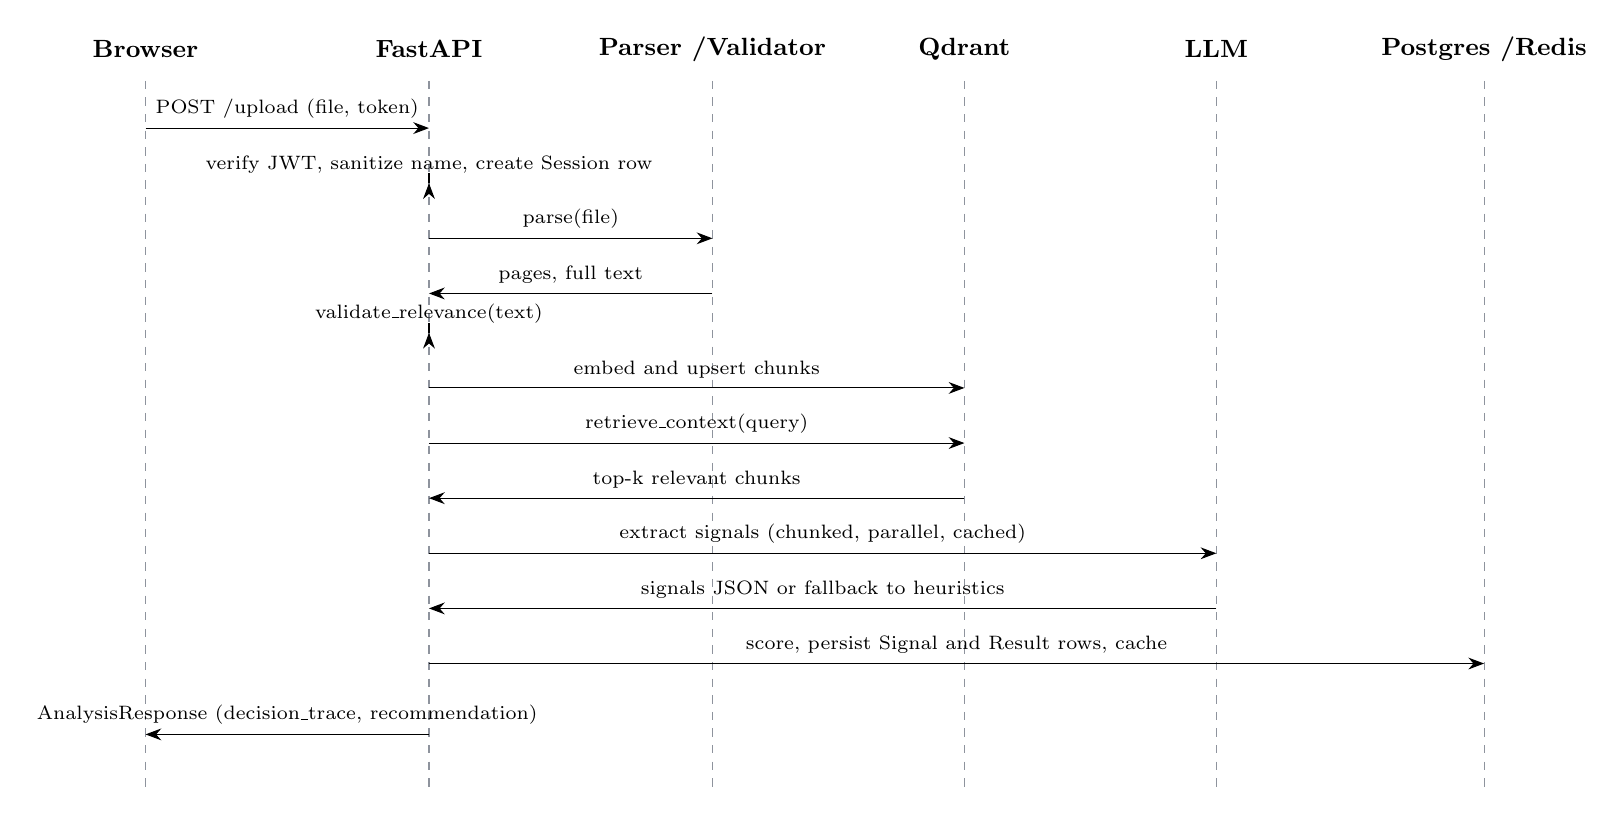
\begin{tikzpicture}[
  actor/.style={font=\small\bfseries},
  lifeline/.style={dashed, draw=darknavy!50},
  msg/.style={-{Stealth[length=2mm]}, font=\scriptsize},
  every node/.style={font=\scriptsize}
]
\def\actorx#1#2{\node[actor] at (#1,0) (#2) {}; \draw[lifeline] (#1,0) -- (#1,-9.6);}
\node[actor] at (0,0) {Browser};
\node[actor] at (3.6,0) {FastAPI};
\node[actor] at (7.2,0) {Parser /\\Validator};
\node[actor] at (10.4,0) {Qdrant};
\node[actor] at (13.6,0) {LLM};
\node[actor] at (17.0,0) {Postgres /\\Redis};
\draw[lifeline] (0,-0.4) -- (0,-9.4);
\draw[lifeline] (3.6,-0.4) -- (3.6,-9.4);
\draw[lifeline] (7.2,-0.4) -- (7.2,-9.4);
\draw[lifeline] (10.4,-0.4) -- (10.4,-9.4);
\draw[lifeline] (13.6,-0.4) -- (13.6,-9.4);
\draw[lifeline] (17.0,-0.4) -- (17.0,-9.4);

\draw[msg] (0,-1.0) -- node[above]{POST /upload (file, token)} (3.6,-1.0);
\draw[msg] (3.6,-1.7) -- node[above]{verify JWT, sanitize name, create Session row} (3.6,-1.7);
\draw[msg] (3.6,-2.4) -- node[above]{parse(file)} (7.2,-2.4);
\draw[msg] (7.2,-3.1) -- node[above]{pages, full text} (3.6,-3.1);
\draw[msg] (3.6,-3.6) -- node[above]{validate\_relevance(text)} (3.6,-3.6);
\draw[msg] (3.6,-4.3) -- node[above]{embed and upsert chunks} (10.4,-4.3);
\draw[msg] (3.6,-5.0) -- node[above]{retrieve\_context(query)} (10.4,-5.0);
\draw[msg] (10.4,-5.7) -- node[above]{top-k relevant chunks} (3.6,-5.7);
\draw[msg] (3.6,-6.4) -- node[above]{extract signals (chunked, parallel, cached)} (13.6,-6.4);
\draw[msg] (13.6,-7.1) -- node[above]{signals JSON or fallback to heuristics} (3.6,-7.1);
\draw[msg] (3.6,-7.8) -- node[above]{score, persist Signal and Result rows, cache} (17.0,-7.8);
\draw[msg] (3.6,-8.7) -- node[above]{AnalysisResponse (decision\_trace, recommendation)} (0,-8.7);
\end{tikzpicture}
\end{center}

\section{Authentication and Ownership Enforcement}

The `verify_firebase_token` dependency is attached, with `auto_error=False`, to routes that support both authenticated and guest access; this lets a route receive either a verified user id or `None`, and apply different logic accordingly (for example, allowing guest sessions to be viewed by anyone who has the analysis id, since no account is associated with them, while strictly checking that an authenticated project's sessions are only accessible to their owning user's Firebase UID). The `_check_session_ownership()` helper in the analysis router centralizes this logic in one place rather than duplicating it across endpoints, an application of the Don't Repeat Yourself principle that also reduces the chance of an authorization bug being introduced in just one of several similar code paths.

\chapter{Database Deep Dive}

\section{Entity Relationship Overview}

\begin{center}
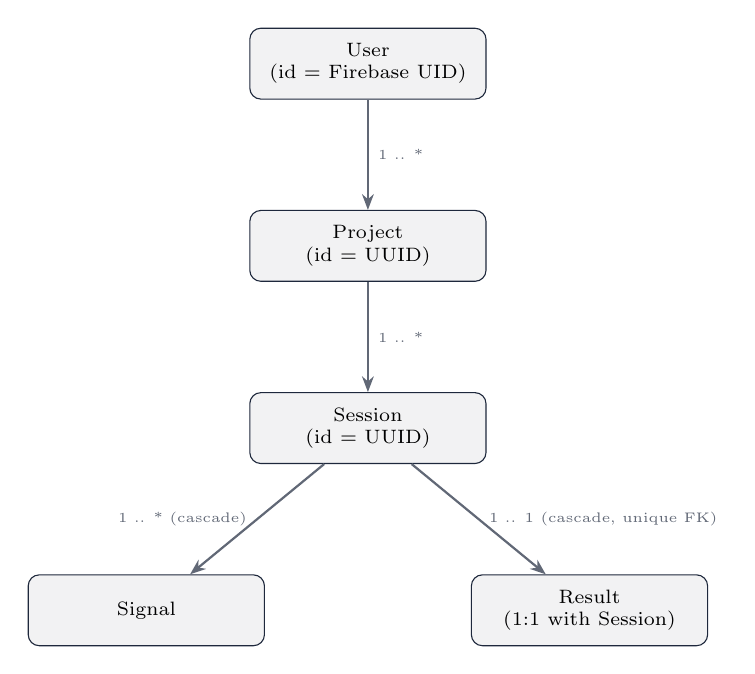
\begin{tikzpicture}[
  ent/.style={rectangle, draw=darknavy, fill=darknavy!6, rounded corners, minimum width=30mm, minimum height=9mm, font=\scriptsize, align=center},
  rel/.style={-{Stealth[length=2mm]}, thick, darknavy!70}
]
\node[ent] (user) {User\\(id = Firebase UID)};
\node[ent, below=14mm of user] (project) {Project\\(id = UUID)};
\node[ent, below=14mm of project] (session) {Session\\(id = UUID)};
\node[ent, below left=14mm and -2mm of session] (signal) {Signal};
\node[ent, below right=14mm and -2mm of session] (result) {Result\\(1:1 with Session)};

\draw[rel] (user) -- node[right,font=\tiny]{1 .. *} (project);
\draw[rel] (project) -- node[right,font=\tiny]{1 .. *} (session);
\draw[rel] (session) -- node[left,font=\tiny]{1 .. * (cascade)} (signal);
\draw[rel] (session) -- node[right,font=\tiny]{1 .. 1 (cascade, unique FK)} (result);
\end{tikzpicture}
\end{center}

\section{Table by Table Schema Walkthrough}

\subsection{User}
Primary key is the Firebase UID itself (a string), avoiding a redundant surrogate key and making lookups by authenticated identity direct. Fields: `name`, `email`, `provider` (the identity provider, for example "google.com"), `photo_url`, and timezone aware `created_at` / `updated_at` timestamps. \textbf{Why this design:} since Firebase is the system of record for identity, mirroring its UID as the primary key avoids a join or lookup table and keeps the relationship between authentication identity and application data direct and obvious.

\subsection{Project}
UUID primary key, a `user_id` foreign key (which may reference a real `User` row or hold a "guest\_" prefixed synthetic identifier for anonymous users, a deliberate, lightweight way to support guest mode without complicating the schema with nullable foreign keys or a separate guest table), `name` (one to sixty characters), `description` (zero to two hundred characters), a `status` field (for example "empty," "in\_progress," "completed"), an optional `analysis_id` pointing at the most recent analysis, and a `mode` field recording whether the project's last analysis used the upload or questionnaire flow.

\subsection{Session}
UUID primary key, a foreign key to `Project` (nullable, supporting guest questionnaire runs that are not attached to any project), a `status` field with the lifecycle values "draft," "processing," "completed," and "error" (the states that the crash recovery logic at startup specifically watches for), the selected LLM `provider`, and the original `filename` for uploaded documents.

\subsection{Signal}
Represents one extracted decision factor for one session: `signal_name` (one of the ten fixed categories), `value`, `confidence` (a float between 0 and 1), `source_text` (the quoted evidence), `page_number`, and `source_verified` (a boolean added in a later migration once the source verification feature was built, demonstrating the schema evolving alongside the feature set). A composite index on `(session_id, signal_name)` makes the very common "fetch all signals for this session" and "fetch this specific signal for this session" queries efficient, and was added explicitly to resolve an "N+1 query" performance issue (tagged "B-11" in the codebase) where signals were previously being fetched one at a time in a loop.

\subsection{Result}
Holds the final, computed recommendation for exactly one session (`session_id` is a unique foreign key, enforcing the one-to-one relationship at the database level): `recommended_architecture`, `confidence_score`, and a set of JSON columns (`ranking`, `scores`, `decision_breakdown`, `why_not`, `suitability`, `followup_questions`, `sensitivity`, `decision_trace`, `architecture_details`) that store the rich, semi structured output of the scoring engine without requiring a sprawling set of additional normalized tables for data that is always read and written as a single cohesive unit.

\section{The PortableJSON Type Decorator}

A custom SQLAlchemy `TypeDecorator` automatically uses PostgreSQL's native, indexable, binary `JSONB` column type in production while falling back to a plain `JSON` (stored as text) column type when running against SQLite, which the test suite uses for fast, dependency free, in-memory database testing. \textbf{Why this matters:} it lets the exact same model definitions be used in both production and tests without conditional code scattered throughout the application, and is a clean example of the Adapter pattern applied at the persistence layer; a candidate should be able to explain that `JSONB` offers indexing and operator support that plain `JSON` does not, which is why the production path prefers it whenever the underlying database supports it.

\section{Cascading Deletes and Referential Integrity}

`Signal` and `Result` rows are configured with cascading deletes tied to their parent `Session`. \textbf{Why this matters:} deleting a session (for example, as part of a project deletion, or a future data retention policy) automatically and atomically removes all of its associated signals and its result, preventing orphaned rows and the bugs and storage waste they would eventually cause, without requiring the application code to remember to clean them up manually in every deletion code path.

\section{Indexing Strategy}

Beyond the composite `(session_id, signal_name)` index on `Signal`, foreign key columns throughout the schema (`Project.user_id`, `Session.project_id`, `Result.session_id`) are individually indexed, since these are the columns most frequently used in `WHERE` clauses and `JOIN` conditions (for example, "all projects for this user," "all sessions for this project," "the result for this session"). \textbf{Tradeoff to be able to discuss:} indexes speed up reads at the cost of slightly slower writes (each insert or update must also update the index) and additional storage; for a read-heavy application like this one, where a given session's data is written once but potentially read many times (every poll, every page reload, every PDF export), this tradeoff clearly favors indexing.

\section{Timezone Handling}

All timestamp columns use `DateTime(timezone=True)` and are populated through a shared `now_utc()` helper, a fix that the codebase notes was applied after discovering inconsistencies between naive and timezone aware datetimes (a notoriously common source of subtle bugs, particularly in systems whose users span multiple time zones, where a naive timestamp's meaning is ambiguous). Storing everything in UTC and converting to the user's local time only at the presentation layer is the standard, correct approach, and this project follows it consistently after the fix was applied.

\end{document}
